\documentclass[11pt]{article}
\usepackage[margin=1in]{geometry}
\usepackage{amsmath,amssymb}
\usepackage{graphicx}
\usepackage{booktabs}
\usepackage[font=small]{caption}
\usepackage[round]{natbib}
\usepackage[hidelinks]{hyperref}

\title{The Instability of Recovery-Trajectory Supervision in Sub-1B Browser Agents}
\author{Mert Dikmen\\\small draft, November 2026}
\date{}

\begin{document}
\maketitle

\begin{abstract}
Training a small browser agent on its own successful trajectories produces a
competent but brittle policy: a single early mistake compounds across the
remaining steps because the model has never been shown how to correct course. A
widely recommended remedy is to supplement the behavioral cloning objective
with recovery trajectories, episodes in which a failure was injected and a
teacher model demonstrated the correction. We evaluate this recipe on a 0.6B
browser agent using a controlled $2\times2$ ablation over the composition of
recovery data, which separates error free steps from error containing steps,
together with a sweep over the fraction of the training set derived from
recovery. Across three to seven seeds per condition, recovery supervision
neither reliably improves the agent nor leaves it unchanged. The full recovery
condition is bimodal across seeds: roughly two of seven runs collapse to a
degenerate policy that issues CLICK actions almost exclusively and never issues
SEARCH or TYPE actions, while the remaining runs track the clean baseline. The
instability is not monotonic in the recovery fraction. It concentrates in a
narrow window near 36 to 40 percent and disappears at both lower and higher
fractions. Validation loss fails to rank checkpoints by task success, and a
collapsed run can achieve the lowest validation loss, whereas a single action
distribution statistic, the fraction of CLICK actions, cleanly separates
healthy from collapsed checkpoints. Checkpoint analysis further shows that the
collapse is a late training bifurcation rather than an early divergence: at
iteration 100 the runs destined to collapse look healthier than several that
eventually recover. We conclude that naive recovery supervision for sub-1B
agents is not merely ineffective but unstable, and that practitioners should
select models for local deployment using multiple seeds and action distribution
monitoring rather than validation loss.
\end{abstract}

\section{Introduction}

Local browser agents, models that run on a laptop without cloud calls, API
costs, or data leaving the device, are a natural fit for sub-1B parameter
models. A 0.6B model fine-tuned on a teacher's successful trajectories reaches
roughly 90 percent on a scoped benchmark, yet the policy it learns remains
brittle. When the model commits an early mistake it rarely recovers, and the
error propagates through the remaining steps of the episode.

The obvious remedy is to teach recovery directly. One collects recovery
trajectories by injecting a failure into an episode, retains the episodes in
which a teacher corrected the failure, and appends these episodes to the
behavioral cloning objective. The appeal is straightforward: the model learns
what to do after an error, not only what to do when everything proceeds as
expected.

Our experiments show that this remedy fails in a specific way at the sub-1B
scale. Recovery supervision has a small and unreliable effect on average
accuracy, but a large effect on variance. A substantial fraction of training
seeds collapse to a degenerate policy, and the collapse is invisible to
validation loss while remaining clearly visible in the distribution of actions
the model emits. We make four contributions.

First, we run a controlled composition ablation that separates error free
recovery steps from error containing recovery steps, and we show that the full
mixture induces bimodal, seed dependent collapse. Second, we run a data mixing
sweep over the recovery derived fraction and find that the effect is
non-monotonic: the collapse occupies a narrow instability window rather than
growing with the amount of recovery data. Third, we show that validation loss
does not rank checkpoints by task success, whereas a single action distribution
statistic, the CLICK share, detects the collapse reliably. This is a practical
model selection signal for agent fine-tuning. Fourth, we trace the collapse to
a late training bifurcation, not an early divergence.

We frame the paper as an empirical characterization rather than a claim of a
new phenomenon. Bimodal seed collapse in small model fine-tuning has already
been reported in knowledge distillation \citep{noisefloor2026} and vision
language action training \citep{vla2026}; recovery annotated trajectories are
deployed at scale by PALADIN \citep{paladin2025}; and masking the error step is
known to help \citep{step2025,srft2026}. Our contribution is the combination of
composition, mixing, and monitoring analysis in the sub-1B browser agent
setting, together with the practical recommendation that follows from it.

\section{Related Work}

\paragraph{Recovery and self correction training.}
\citet{paladin2025} train on more than fifty thousand recovery annotated
trajectories constructed through systematic failure injection and LoRA
fine-tuning, and report substantial gains in recovery rate. \citet{step2025}
and \citet{srft2026} mask the error step and train only on the correction,
finding that masking helps. These methods operate at a scale and with reasoning
channels that we do not use, and none of them report seed level instability. We
study the small data sub-1B regime in which the effect becomes unreliable.

\paragraph{Bimodal seed collapse.}
\citet{noisefloor2026} document bimodal seed collapse in small model knowledge
distillation, where one in three to two in five seeds falls below 55 percent
accuracy while the rest train normally, and distinguish several collapse modes.
\citet{vla2026} report the same seed lottery in vision language action
fine-tuning. Our work reproduces this phenomenon in a different setting,
recovery data supervised fine-tuning for browser tool use, and connects it to a
monitoring signal, the action distribution, rather than to a training
objective.

\paragraph{SFT, data distribution, and label prior.}
\citet{sftmemorizes2025} argue that supervised fine-tuning imprints the training
distribution, and label prior bias is a recognized failure mode of imbalanced
fine-tuning \citep{labelbias2024}. The CLICK only collapse we observe is an
instance of this label prior imprinting acting on the action space rather than
on a label space.

\paragraph{Small model tool use SFT.}
\citet{sftorrl2026} find that LoRA supervised fine-tuning is the strongest in
distribution method for tool calling from 0.6B to 32B parameters. We hold the
pipeline fixed and vary only the composition of the recovery data.

\section{Method}

\subsection{Benchmark}
We use a 51 task browser benchmark with programmatic oracles spanning four
categories: navigation (10 tasks), search (9), form filling (19), and
multi-step (13). Tasks run against static fixtures through Playwright, and
success is determined by the oracle rather than by a language model judge. A
separate 10 task held out set on an unseen site serves as a secondary
generalization check.

\subsection{Data}
A Qwen3 4B teacher generates successful trajectories, which we convert into
single turn supervised fine-tuning examples of the form (observation, action).
We collect two pools. The clean pool contains trajectories with no injected
failure. The recovery pool contains trajectories in which we injected a stale
observation failure, removing an element so that every subsequent reference
shifts, and in which the teacher recovered. Each recovery trajectory
contributes two kinds of step. Error free steps, which we call clean like, are
the actions before the injection and after the recovery and resemble ordinary
clean data. Error containing steps, which we call recovery signal, are the
steps whose observation carries the injected error.

\subsection{Composition ablation}
From a fixed clean set of 84 examples we build four conditions: A holds 84 clean
examples; B adds 34 clean like examples; C adds 21 recovery signal examples; D
adds all 55 recovery derived examples.

\subsection{Data mixing sweep}
Holding the recovery composition fixed, we vary the recovery derived fraction
across 0, 20, 29, 33, 36, 40, 46, and 50 percent. Fractions above 40 percent are
achieved by subsampling the clean set, a confound we flag in Section 5.

\subsection{Training and evaluation}
We fine-tune Qwen3 0.6B with LoRA (rank 8, 16 layers), batch size 4, 200
iterations, learning rate $10^{-4}$, assistant token only loss, and no thinking
channel. Each condition uses three to seven seeds. For every run we record task
success, per category success, the full action sequence for the CLICK, TYPE,
SEARCH, and SUBMIT distribution, validation loss, and the iteration 100
checkpoint.

\section{Results}

\subsection{Bimodal outcomes in the full recovery condition}
Table~\ref{tab:seeds} reports per seed results. Conditions A and B are unimodal
and stable. Condition D is bimodal: two seeds collapse to 16 and 27 while five
sit between 38 and 47.

\begin{table}[h]
\centering
\caption{Task success on the 51 task benchmark, per seed.}
\label{tab:seeds}
\begin{tabular}{lcccc}
\toprule
Condition & $n$ & Mean $\pm$ std & Range \\
\midrule
A (clean) & 7 & $45.7 \pm 2.9$ & 40 to 49 \\
B (plus clean like) & 6 & $47.2 \pm 3.6$ & 43 to 51 \\
C (plus recovery) & 7 & $40.9 \pm 5.4$ & 31 to 46 \\
D (both) & 7 & $36.6 \pm 11.2$ & \textbf{16 to 47} \\
\bottomrule
\end{tabular}
\end{table}

When the collapse occurs it takes a consistent form, which we detail in
Section~\ref{sec:attractor}: roughly 94 percent CLICK, zero SEARCH, zero SUBMIT,
and a rise in steps per task from 2.8 to 5.1.

\subsection{Non-monotonic data mixing}
Table~\ref{tab:mix} and Figure~\ref{fig:mixing} show that the instability
concentrates in a window near 36 to 40 percent and is not monotonic. Higher
recovery fractions do not produce more collapse. The collapse modes also vary
across seeds: one seed collapses broadly, another collapses only on search, and
the CLICK only mode of Section~\ref{sec:attractor} is a third distinct form. The
failure is therefore not a single mechanism.

\begin{table}[h]
\centering
\caption{Recovery derived fraction against task success.}
\label{tab:mix}
\begin{tabular}{lcccc}
\toprule
Fraction & $n$ & Mean $\pm$ std & Collapse \\
\midrule
0\% & 7 & $45.7 \pm 2.9$ & none \\
20\% & 7 & $40.9 \pm 5.4$ & none \\
29\% & 6 & $47.2 \pm 3.6$ & none \\
33\% & 3 & $41.0 \pm 2.6$ & none \\
36\% & 3 & $41.3 \pm 13.3$ & 1 of 3 \\
40\% & 7 & $36.6 \pm 11.2$ & 2 of 7 \\
46\% & 3 & $42.7 \pm 4.5$ & none \\
50\% & 3 & $43.0 \pm 1.7$ & none \\
\bottomrule
\end{tabular}
\end{table}

\begin{figure}[h]
\centering
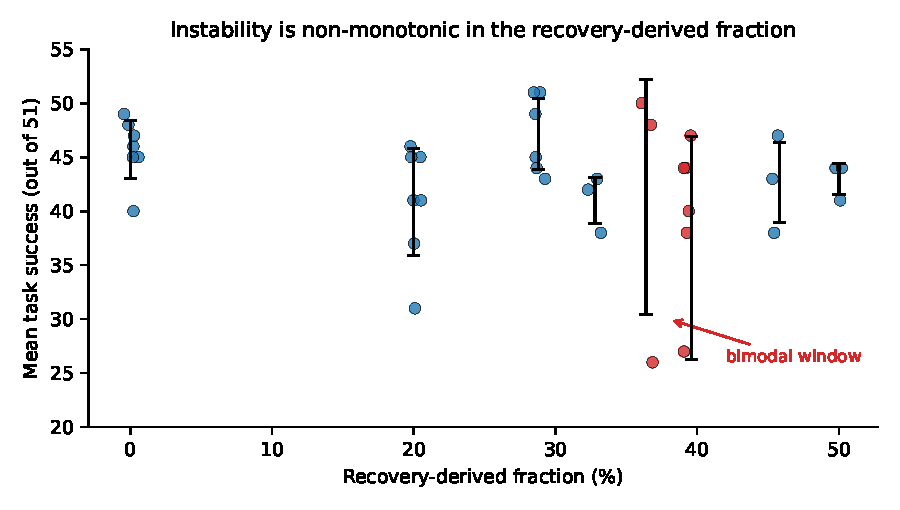
\includegraphics[width=0.7\linewidth]{figures/fig2_mixing.pdf}
\caption{The instability is non-monotonic in the recovery derived fraction; the
collapse concentrates in a narrow window.}
\label{fig:mixing}
\end{figure}

\subsection{The CLICK only attractor and action monitoring}
\label{sec:attractor}
Table~\ref{tab:actions} and Figure~\ref{fig:actions} report the action
distribution on the clean 51 task run. A high CLICK share alone is not fatal;
condition B succeeds at 59 percent CLICK. What distinguishes the collapsed runs
is the loss of the other action types. This makes the CLICK share, or
equivalently the presence of SEARCH and TYPE, a cheap and interpretable monitor
of collapse.

\begin{table}[h]
\centering
\caption{Action distribution on the clean 51 task run.}
\label{tab:actions}
\begin{tabular}{lccc}
\toprule
Model & CLICK & TYPE & SEARCH \\
\midrule
A & 29.1\% & 59.6\% & 3.5\% \\
B & 59.3\% & 32.1\% & 5.7\% \\
C & 29.9\% & 51.3\% & 3.6\% \\
D (healthy seed) & 59.7\% & 27.6\% & 6.0\% \\
D (collapsed seed) & \textbf{93 to 95\%} & \textbf{0 to 7\%} & \textbf{0\%} \\
\bottomrule
\end{tabular}
\end{table}

\begin{figure}[h]
\centering
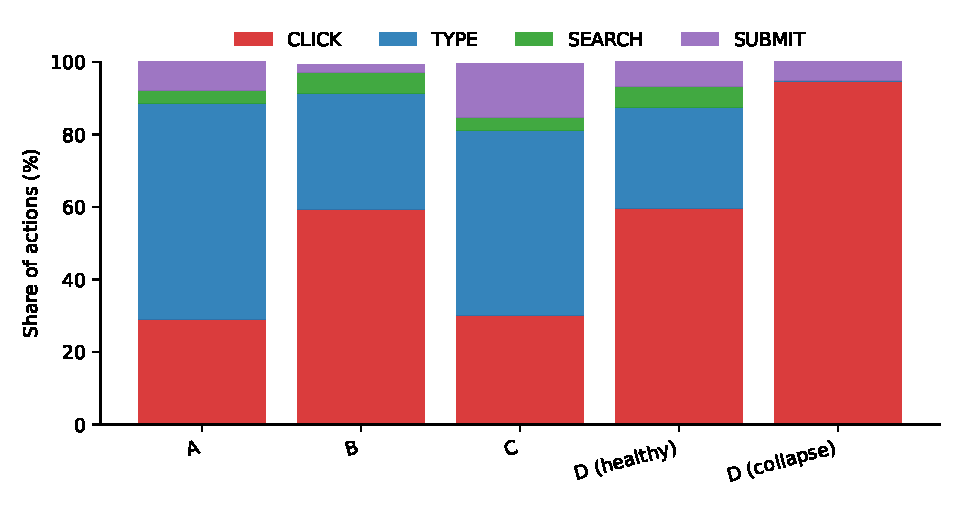
\includegraphics[width=0.8\linewidth]{figures/fig3_actions.pdf}
\caption{Action distribution. Collapsed D seeds lose SEARCH and TYPE entirely.}
\label{fig:actions}
\end{figure}

\subsection{Validation loss is blind to the collapse}
Figure~\ref{fig:valloss} plots validation loss against task success across all
seeds. Validation loss does not rank checkpoints. A collapsed D seed scoring 16
of 51 achieves a validation loss of 0.178, which is lower than the best healthy
seed at 47 of 51 with a loss of 0.217. The validation split contains roughly 14
examples and is dominated by clean data, so it cannot see the action
distribution pathology. The CLICK share, by contrast, cleanly separates
collapsed from healthy checkpoints at 93, 60, and 30 percent.

\begin{figure}[h]
\centering
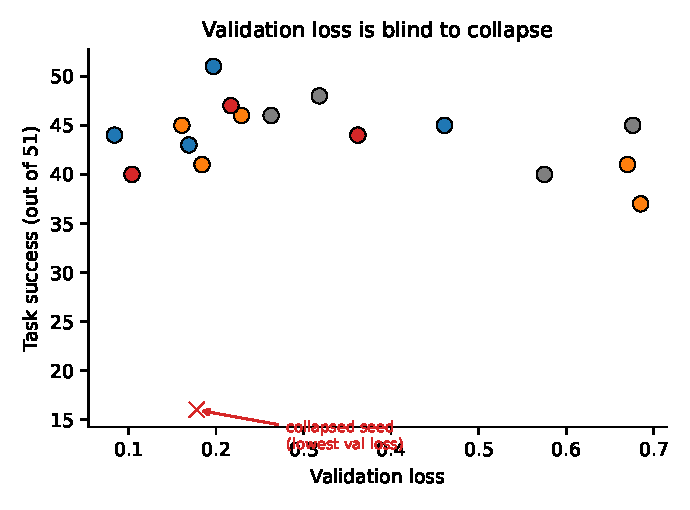
\includegraphics[width=0.55\linewidth]{figures/fig4_valloss.pdf}
\caption{Validation loss against task success. A collapsed seed achieves the
lowest validation loss, so validation loss is blind to the collapse.}
\label{fig:valloss}
\end{figure}

\subsection{A late training bifurcation}
Figure~\ref{fig:dynamics} compares iteration 100 with final success for the five
D seeds. At iteration 100 the seeds destined to collapse look healthier than
several that eventually recover: the collapsing seeds score 30 to 32 of 51 with
low CLICK, while two healthy seeds are already CLICK dominant at 62 and 100
percent. The collapse therefore develops in the second half of training. The
model traverses a transient CLICK phase and either escapes it or is captured by
it.

\begin{figure}[h]
\centering
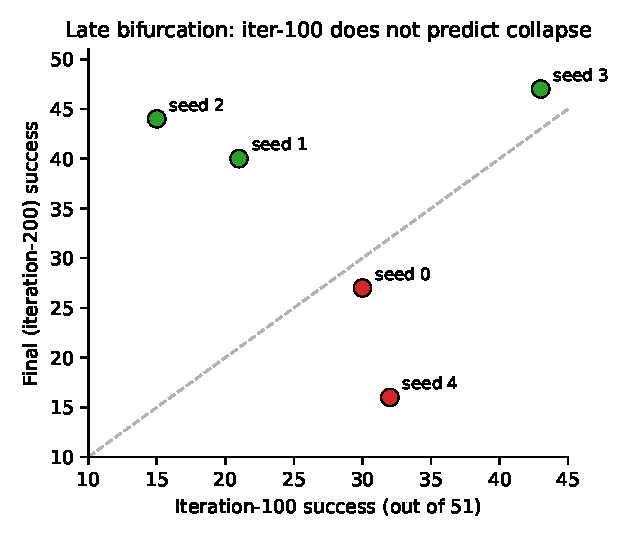
\includegraphics[width=0.55\linewidth]{figures/fig5_dynamics.pdf}
\caption{Iteration 100 against final success for condition D. Red points
collapse; iteration 100 performance does not predict the collapse.}
\label{fig:dynamics}
\end{figure}

\section{Discussion}

\paragraph{Mechanism.}
The CLICK only collapse is consistent with label prior imprinting. A recovery
set that is 71 percent CLICK biases the policy toward CLICK, and once SEARCH and
TYPE are driven out of the action distribution the policy becomes trapped in a
loop. We offer this as a hypothesis. The action distribution evidence is
consistent with it but does not establish causation.

\paragraph{Relation to prior work.}
We do not claim to discover bimodal collapse, which \citet{noisefloor2026}
already documented, nor do we claim that recovery data cannot help, which
\citet{paladin2025} shows it can at scale. Our contribution is the controlled
composition, mixing, and monitoring analysis in the sub-1B browser setting, and
the action distribution signal that detects collapse where validation loss
cannot.

\paragraph{Practical recommendations.}
Practitioners training local sub-1B agents should not assume that recovery data
helps. They should validate with multiple seeds rather than one, monitor the
action distribution rather than validation loss when selecting a checkpoint, and
treat the recovery derived fraction conservatively, since the instability
concentrates in a narrow window.

\paragraph{Limitations.}
The benchmark is synthetic and confined to a single domain. The model family is
a single Qwen3 checkpoint. Seed counts are small, between three and seven. The
46 and 50 percent mixing points are confounded by clean subsampling. The
mechanism is correlational rather than causal. The held out set is too small to
support strong generalization claims.

\section{Conclusion}
Recovery trajectory supervision for sub-1B browser agents has a small and
unreliable mean effect but produces bimodal, seed dependent outcomes. A subset
of seeds collapse to a CLICK only policy that validation loss fails to detect,
while a single action distribution statistic reveals it. The instability is
non-monotonic in the recovery derived fraction and reflects a late training
bifurcation. For local agent training, the quantity that matters is stability,
and it should be assessed with multiple seeds and action distribution monitoring
rather than validation loss.

\begin{thebibliography}{99}
\bibitem[Sumit et al.(2026)]{noisefloor2026}
Sumit et al. Below the noise floor: Bimodal seed collapse and distinct failure
modes in small-model knowledge distillation. arXiv:2608.27729, 2026.

\bibitem[VLA(2026)]{vla2026}
Output-level regularization eliminates the seed lottery in single-GPU VLA
fine-tuning. arXiv:2606.13856, 2026.

\bibitem[Vuddanti et al.(2025)]{paladin2025}
PALADIN: Self-correcting language model agents to cure tool-failure cases.
arXiv:2509.25238, 2025.

\bibitem[Chen et al.(2025)]{step2025}
Chen et al. Training LLM-based agents with synthetic self-reflected trajectories
and partial masking. arXiv:2505.20023, 2025.

\bibitem[SRFT(2026)]{srft2026}
Step rejection fine-tuning: Squeezing more signal from noisy agent trajectories.
JetBrains Research, 2026.

\bibitem[SFT-RL(2025)]{sftmemorizes2025}
SFT memorizes, RL generalizes: A comparative study of foundation model
post-training. ICML, 2025. arXiv:2501.17161.

\bibitem[Label Bias(2024)]{labelbias2024}
Beyond performance: Quantifying and mitigating label bias in LLMs. NAACL, 2024.
arXiv:2405.02743.

\bibitem[SFT-or-RL(2026)]{sftorrl2026}
SFT or RL for tool-calling agents? A controlled study across data, method, and
scale. arXiv:2609.17848, 2026.
\end{thebibliography}

\end{document}
